\section{Effects on Users} \label{sec:users}
Every user can store a maximum amount of  news, i.e. has a memory: this distinctive trait could affect news' distribution among users.
Indeed, if we insert in the network a certain number of news
(i.e. launching a simulation with many news), they will reach a
fraction of users (\textit{FOUR}, fraction of users reached)
at a fixed time.
\footnote{20 news for all of our simulations.}\\
News spreading over time, in general, starts with a fluctuating
transient and then reaches a stationary state: from a ``microscopic''
point of view, users' identity might vary but the fraction is
pretty much the same. \\
It is statistically correct to compute, for every news, the average
\textit{FOUR} over time, with a given threshold in order to
neglect the transient.\footnote{The end time and the threshold are
  experimentally determined by free trials. Moreover, threshold is
  not statistically significant since the end time was several orders of magnitude higher.}
Proceding this way, we obtain a distribution of average \textit{FOURs}
for each news.\\
\subsection{Gini Index}
\textit{Gini index}\cite{ginindex} measures the inequality of a
distribution. Values of 0 and 1 stand for, respectively, the
maximum homogeneity and the maximum heterogeneity.
However, this index is a function of random values: mean and
error have to be estimated.\\
A certain number of samples is created by sampling with replacement
of the average FOUR distribution: Gini index is computed for each
one of them.
Now we have a population of Gini indexes, and we can extract
mean and error: the whole process is known as
\textit{bootstrap}\cite{bootstrap}
(see \hl{Appendix 1} for error estimation).\\
In practical terms, for every level of  memory, a simulation with
twenty news is run out: Gini index' mean and error are computed
like before.
The Gini index-memory plot shows a highly non-linear behaviour:
sigmoid and gaussian seem to better represent data.\\
In order to select the best-fit function, \textit{Chi-square} is
computed for both of them. \\
Because of asymmetric error bars, the optimization function is
slightly different from the standard one, used for weighted
interpolation: see \hl{Appendix 2} for more details.
Interpolation results are shown below:

%\begin{figure}[!h]
  %\centering
  %\includegraphics[width=.7\columnwidth]{img/gini_memory.png}
  %\caption{Gini index-memory plot with errorbars}
  %\label{fig:ginimem}
%\end{figure}




\begin{figure}[h]
  \centering
  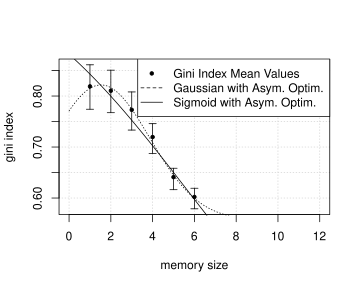
\includegraphics[trim={0cm 0cm 0cm 1cm},clip,width=.8\columnwidth]{img/gini.pdf}
  \caption{Gini index on memory size.}
  \label{fig:gini}
\end{figure}

\begin{table}[h]
  \centering
  \begin{tabular}{rSSSS}
    \toprule
    & \multicolumn{2}{c}{\textit{Gaussian Fit}} & \multicolumn{2}{c}{\textit{Sigmoid Fit}}\\
     & {$\chi^2$} & {p-value} & {$\chi^2$} & {p-value} \\ \midrule
    stde & 0.0013260 & 0.97195 & 0.00080793 & 0.97732 \\
    qant & 0.0037563 & 0.95113 & 0.0012997  & 0.97124 \\
    asym & 0.0013576 & 0.97061 & 0.00084281 & 0.97684 \\ \bottomrule
  \end{tabular}
  \caption{Reduced $\chi^2$ and respective p-value for Gaussian
    and Sigmoid fit with different non-linear optimization
    strategies.\\
    Optimization using the standard error of the Gini index
    is denoted as std, quantile bootstrap optimization\cite{quantile} as
    quant and asymmetric error bar fitting optimization as asym.}
  \label{tab:gini}
\end{table}

We can notice that, for every type of errorbar, sigmoid's
$\chi^2$ is slightly lower than gaussian one; p-value is
higher instead.
Null hypothesis, for both measures, is far from being rejected:
goodness-of-fit is solidly validated.
Hence, sigmoid is our best-fit function for gini index-memory
length plot.

\subsection{Echo chambers}
In news media, \textit{echo chamber} is a metaphorical description
of a situation in which beliefs are amplified or reinforced by
communication and repetition inside a closed system\cite{echochamwiki,echocham}.\\
We qualitatively investigated the presence of echo chambers in our network.
First of all, our agents have a ``mental  state'', i.e. a vector of preferences: its components represent the amount of interest toward a certain topic.\\
 News have the same dimension of \textit{mental state vector} (MSVD) in order to establish a ``matching'' between news' topics and users' preferences.
 Mental state is highly involved in news' dynamics and network topology.\footnote{See section~\ref{introduction} for more details on the previous work.}\\
 In the images below, for MSVD=3,5,7, we extracted main clusters from our network.
 Memory length is twelve for all the simulations.\\
 \textit{Modularity} is a measure for detecting community structure in graphs\cite{modulwiki}.
 To provide a comparison, nodes were painted with modularity class and the most recent news in memory.
 In case of news' homogeneity inside a single cluster, we are observing an echo chamber.\\
We can notice that number of clusters equals MSVD basically.
News' situation is more heterogenous: altough some clusters still exist, there is not a clear separation among users with different news.


\begin{figure}

  \centering
  \begin{subfigure}[t]{0.25\textwidth}
    \includegraphics[width=\textwidth]{img/dim3_mod.pdf}
    \label{fig:bubble3mod}
    \caption{}
  \end{subfigure}
  ~
  \begin{subfigure}[t]{0.35\textwidth}
    \includegraphics[width=\textwidth]{img/dim5_mod.pdf}
    \label{fig:bubble5mod}
    \caption{bubble3news}
  \end{subfigure}
  ~
  \begin{subfigure}[t]{0.35\textwidth}
    \includegraphics[width=\textwidth]{img/dim7_mod.pdf}
    \label{fig:bubble7mod}
    \caption{bubble3news}
  \end{subfigure}
  \\
  \begin{subfigure}[t]{0.25\textwidth}
    \includegraphics[width=\textwidth]{img/dim3_news.pdf}
    \label{fig:bubble3news}
    \caption{bubble3mod}
  \end{subfigure}
  ~
  \begin{subfigure}[t]{0.35\textwidth}
    \includegraphics[width=\textwidth]{img/dim5_news.pdf}
    \label{fig:bubble5news}
    \caption{bubble3news}
  \end{subfigure}
  ~
  \begin{subfigure}[t]{0.35\textwidth}
    \includegraphics[width=\textwidth]{img/dim7_news.pdf}
    \label{fig:bubble5news}
    \caption{bubble3news}
  \end{subfigure}
  \caption{Simulations for 1000 users and 20 sources after 1000
    iterations. (\ref{fig:bubble3mod}), (\ref{fig:bubble5mod}) and
    (\ref{fig:bubble7mod}) highlights state vector.
    (\ref{fig:bubble3news}), (\ref{fig:bubble3news}) and
    (\ref{fig:bubble3news}) hightlitghts different news.
}
  \label{fig:test}
\end{figure}
